\chapter{Đọc thêm 1: Định lượng Hành vi Giao dịch qua Google Trends (Preis, Moat \& Stanley)}
\label{ch:M4L2DT1}

% Nguồn: Preis, T., Moat, H. S., & Stanley, H. E. ``Quantifying Trading Behavior in Financial Markets Using Google Trends.'' Scientific Reports, 3(1), 2013.
% Phần cần đọc: Toàn bộ bài báo
% Nội dung bắt buộc đọc: được kiểm tra trong mọi bài đánh giá (kể cả Quiz).

\section{Thông tin nguồn}

\begin{itemize}
  \item \textbf{Nguồn:} Preis, T., Moat, H. S., and Stanley, H. E. \emph{Quantifying Trading Behavior in Financial Markets Using Google Trends}. Scientific Reports, 3(1), 2013. \url{https://doi.org/10.1038/srep01684}
  \item \textbf{Phần cần đọc:} Toàn bộ nội dung
\end{itemize}

\subsection*{Thông tin bài báo}

\begin{itemize}
  \item \textbf{Tiêu đề gốc:} Quantifying Trading Behavior in Financial Markets Using Google Trends
  \item \textbf{Tác giả:} Tobias Preis\textsuperscript{1*}, Helen Susannah Moat\textsuperscript{2,3*} \& H. Eugene Stanley\textsuperscript{2*}
  \item \textbf{Đơn vị công tác:} (1) Warwick Business School, University of Warwick, Scarman Road, Coventry, CV4 7AL, Vương quốc Anh; (2) Department of Physics, Boston University, 590 Commonwealth Avenue, Boston, Massachusetts 02215, Hoa Kỳ; (3) Department of Civil, Environmental and Geomatic Engineering, UCL, Gower Street, London, WC1E 6BT, Vương quốc Anh. (* Các tác giả này đóng góp ngang nhau cho công trình này.)
  \item \textbf{Lĩnh vực chuyên môn:} Vật lý thống kê, nhiệt động lực học và động lực học phi tuyến; Vật lý ứng dụng; Khoa học tính toán; Lý thuyết thông tin và tính toán
  \item \textbf{Ngày nhận bài:} 25/02/2013 \quad \textbf{Ngày chấp nhận:} 03/04/2013 \quad \textbf{Ngày xuất bản:} 25/04/2013
  \item \textbf{Liên hệ:} Tobias Preis (Tobias.Preis@wbs.ac.uk)
\end{itemize}

\section{Trích yếu}

Các cuộc khủng hoảng trên thị trường tài chính ảnh hưởng đến con người trên toàn thế giới. Dữ liệu thị trường chi tiết về các quyết định giao dịch phản ánh một phần hành vi phức tạp của con người vốn đã dẫn đến những cuộc khủng hoảng này. Chúng tôi cho rằng các nguồn dữ liệu mới quy mô lớn xuất phát từ tương tác của con người với Internet có thể mang lại một góc nhìn mới về hành vi của những người tham gia thị trường trong các giai đoạn thị trường biến động mạnh. Bằng cách phân tích những thay đổi trong khối lượng truy vấn Google đối với các từ khóa tìm kiếm liên quan đến tài chính, chúng tôi phát hiện ra các mô hình có thể được diễn giải như những ``dấu hiệu cảnh báo sớm'' về các biến động của thị trường chứng khoán. Kết quả của chúng tôi minh họa tiềm năng mà việc kết hợp các tập dữ liệu hành vi quy mô lớn mang lại cho việc hiểu rõ hơn về hành vi tập thể của con người.

\section{Giới thiệu}

Khối lượng ngày càng tăng của ``dữ liệu lớn'' phản ánh nhiều khía cạnh khác nhau trong các hoạt động thường ngày của chúng ta đang mang lại một cơ hội mới then chốt để các nhà khoa học giải quyết những câu hỏi nền tảng về thế giới phức tạp mà chúng ta đang sống. Thị trường tài chính là một mục tiêu hàng đầu cho các nghiên cứu định lượng như vậy. Các biến động trên thị trường gây ra những tác động to lớn đến tài sản cá nhân và các sự kiện địa chính trị, khiến chủ đề này thu hút sự quan tâm đáng kể của giới khoa học. Chẳng hạn, một loạt nghiên cứu gần đây đã tập trung vào việc mô hình hóa thị trường tài chính và thực hiện các phân tích mạng lưới.

Về bản chất, các tập dữ liệu giao dịch tài chính phản ánh vô số quyết định được đưa ra bởi những người tham gia thị trường. Theo Herbert Simon, các chủ thể bắt đầu quá trình ra quyết định của mình bằng cách cố gắng thu thập thông tin. Trong thế giới ngày nay, việc thu thập thông tin thường bao gồm việc tìm kiếm trên các nguồn trực tuyến. Gần đây, công cụ tìm kiếm Google đã bắt đầu cung cấp quyền truy cập vào thông tin tổng hợp về khối lượng truy vấn đối với các từ khóa tìm kiếm khác nhau và cách các khối lượng này thay đổi theo thời gian, thông qua dịch vụ công khai Google Trends. Trong nghiên cứu này, chúng tôi tìm hiểu khả năng thú vị của việc phân tích dữ liệu truy vấn tìm kiếm từ Google Trends nhằm mang lại những hiểu biết mới về quá trình thu thập thông tin diễn ra trước các quyết định giao dịch được ghi nhận trong dữ liệu thị trường chứng khoán.

Một nghiên cứu gần đây đã chỉ ra rằng số lượt nhấp chuột vào kết quả tìm kiếm xuất phát từ một quốc gia nhất định có tương quan với lượng đầu tư vào quốc gia đó. Các nghiên cứu khác khai thác chiều thời gian của dữ liệu Google Trends đã chứng minh rằng những thay đổi trong khối lượng truy vấn đối với các từ khóa tìm kiếm được chọn phản ánh những thay đổi trong số ca nhiễm cúm hiện tại và khối lượng giao dịch hiện tại trên thị trường chứng khoán. Việc chứng minh mối liên hệ giữa khối lượng giao dịch thị trường chứng khoán và khối lượng tìm kiếm cũng đã được lặp lại bằng cách sử dụng dữ liệu của Yahoo!. Choi và Varian đã chỉ ra rằng dữ liệu từ Google Trends có thể được liên kết với giá trị hiện tại của nhiều chỉ số kinh tế khác nhau, bao gồm doanh số bán ô tô, số đơn xin trợ cấp thất nghiệp, việc lên kế hoạch cho điểm đến du lịch và niềm tin tiêu dùng. Một nghiên cứu rất gần đây đã chỉ ra rằng người dùng Internet ở các quốc gia có GDP bình quân đầu người cao hơn có xu hướng tìm kiếm thông tin về những năm trong tương lai nhiều hơn là những năm trong quá khứ.

Ở đây, chúng tôi cho rằng trong khoảng thời gian nghiên cứu, dữ liệu Google Trends không chỉ phản ánh trạng thái hiện tại của thị trường chứng khoán mà còn có thể đã dự báo được một số xu hướng tương lai nhất định. Các phát hiện của chúng tôi phù hợp với đề xuất thú vị rằng những đợt sụt giảm đáng chú ý trên thị trường tài chính thường được báo trước bởi các giai đoạn lo ngại của nhà đầu tư. Trong những giai đoạn như vậy, nhà đầu tư có thể tìm kiếm thêm thông tin về thị trường trước khi cuối cùng quyết định mua hoặc bán. Kết quả của chúng tôi cho thấy rằng, theo logic này, trong giai đoạn từ năm 2004 đến năm 2011, khối lượng truy vấn tìm kiếm Google Trends đối với một số từ khóa nhất định có thể đã được sử dụng trong việc xây dựng các chiến lược giao dịch có lợi nhuận.

\section{Kết quả}

Chúng tôi phân tích hiệu suất của một tập hợp gồm 98 từ khóa tìm kiếm. Chúng tôi đưa vào các từ khóa liên quan đến khái niệm thị trường chứng khoán, với một số từ khóa được gợi ý bởi dịch vụ Google Sets, một công cụ xác định các từ khóa có liên quan về mặt ngữ nghĩa. Do đó, tập hợp từ khóa được sử dụng không được lựa chọn một cách ngẫu nhiên, vì chúng tôi đã chủ ý đưa vào một độ lệch mang tính tài chính. Chúng tôi giải thích chiến lược của mình dựa trên những thay đổi trong khối lượng tìm kiếm bằng cách lấy từ khóa \emph{debt} làm ví dụ tham chiếu, một từ khóa có mối liên hệ ngữ nghĩa rõ ràng với cuộc khủng hoảng tài chính gần đây nhất, và nhìn chung đây cũng là từ khóa cho hiệu suất tốt nhất trong các phân tích của chúng tôi.

\begin{figure}[H]
\centering
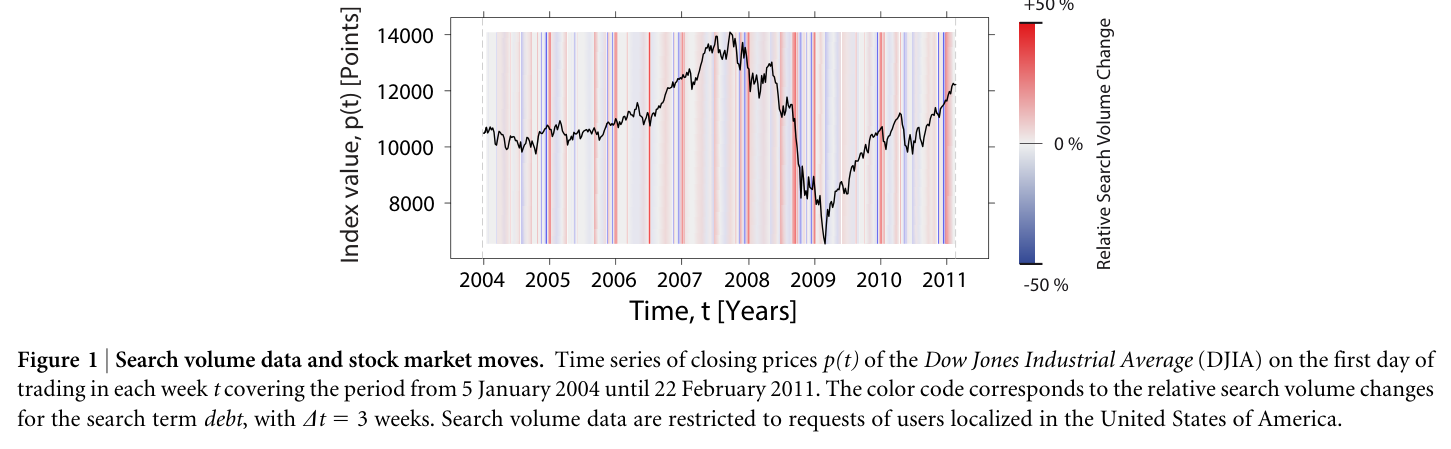
\includegraphics[width=0.8\linewidth]{gfx/m4l2_preis_fig1_search_volume_stock_moves.png}
\par\smallskip{\small \textbf{Hình 1:} Dữ liệu khối lượng tìm kiếm và các biến động của thị trường chứng khoán. Chuỗi thời gian giá đóng cửa $p(t)$ của chỉ số công nghiệp trung bình Dow Jones (DJIA) vào ngày giao dịch đầu tiên của mỗi tuần $t$, trong giai đoạn từ ngày 5 tháng 1 năm 2004 đến ngày 22 tháng 2 năm 2011. Mã màu tương ứng với sự thay đổi tương đối của khối lượng tìm kiếm đối với từ khóa \emph{debt}, với $\Delta t = 3$ tuần. Dữ liệu khối lượng tìm kiếm được giới hạn ở các yêu cầu tìm kiếm của người dùng tại Hoa Kỳ.}
\end{figure}

Để làm sáng tỏ mối quan hệ giữa khối lượng truy vấn tìm kiếm đối với một từ khóa cụ thể và hướng đi chung trong quyết định của nhà giao dịch, chúng tôi phân tích giá đóng cửa $p(t)$ của chỉ số DJIA vào ngày giao dịch đầu tiên của tuần $t$. Chúng tôi sử dụng Google Trends để xác định số lượt tìm kiếm $n(t-1)$ đã được thực hiện đối với một từ khóa cụ thể, chẳng hạn như \emph{debt}, trong tuần $t-1$ (Google định nghĩa một tuần kết thúc vào ngày Chủ nhật), tính theo tỷ lệ so với tổng số lượt tìm kiếm được thực hiện trên Google trong khoảng thời gian đó. Chúng tôi nhận thấy rằng dữ liệu khối lượng tìm kiếm thay đổi nhẹ theo thời gian do quy trình trích xuất của Google. Do đó, đối với mỗi từ khóa tìm kiếm, chúng tôi lấy trung bình của ba lần thực hiện chuỗi thời gian khối lượng tìm kiếm của từ khóa đó, dựa trên ba yêu cầu dữ liệu độc lập trong các tuần liên tiếp. Sự biến thiên của dữ liệu Google Trends theo các ngày truy cập khác nhau không ảnh hưởng đến kết quả của chúng tôi, và có thể chứng minh rằng dữ liệu này phù hợp với các sự kiện thực tế đã được ghi nhận (xem Hình S1 trong Thông tin Bổ sung).

Để định lượng những thay đổi trong hành vi thu thập thông tin, chúng tôi sử dụng độ thay đổi tương đối của khối lượng tìm kiếm:
$$
\Delta n(t, \Delta t) = n(t) - N(t-1, \Delta t)
$$
với
$$
N(t-1, \Delta t) = \frac{n(t-1) + n(t-2) + \cdots + n(t-\Delta t)}{\Delta t}
$$
trong đó $t$ được đo bằng đơn vị tuần. Trong Hình 1, chúng tôi biểu diễn sự thay đổi tương đối của khối lượng tìm kiếm đối với từ khóa \emph{debt}, cùng với mối quan hệ của nó với giá đóng cửa của DJIA.

Để tìm hiểu xem những thay đổi trong hành vi thu thập thông tin được ghi nhận qua dữ liệu Google Trends có liên quan đến những thay đổi giá cổ phiếu sau đó trong giai đoạn 2004--2011 hay không, chúng tôi xây dựng một chiến lược đầu tư giả định cho một danh mục sử dụng dữ liệu khối lượng tìm kiếm, gọi là ``chiến lược Google Trends'' trong phần tiếp theo. Lợi nhuận chỉ có thể đạt được trong một chiến lược giao dịch nếu ít nhất một số thay đổi tương lai của giá cổ phiếu được dự đoán đúng, đặc biệt là xung quanh các biến động lớn của thị trường. Chúng tôi thực hiện chiến lược này bằng cách bán DJIA tại giá đóng cửa $p(t)$ vào ngày giao dịch đầu tiên của tuần $t$, nếu $\Delta n(t-1, \Delta t) > 0$, và mua lại DJIA tại giá $p(t+1)$ vào cuối ngày giao dịch đầu tiên của tuần kế tiếp. Lưu ý rằng có tồn tại các cơ chế cho phép bán tài sản trên thị trường tài chính mà không cần sở hữu tài sản đó trước. Ngược lại, nếu $\Delta n(t-1, \Delta t) < 0$, chúng tôi mua DJIA tại giá đóng cửa $p(t)$ vào ngày giao dịch đầu tiên của tuần $t$ và bán DJIA tại giá $p(t+1)$ vào cuối ngày giao dịch đầu tiên của tuần tiếp theo. Tại thời điểm bắt đầu giao dịch, chúng tôi đặt giá trị của tất cả các danh mục ở một mức tùy ý là 1. Nếu chúng tôi thực hiện một vị thế bán khống (short position), tức bán tại giá đóng cửa $p(t)$ và mua lại tại giá $p(t+1)$, thì lợi suất tích lũy $R$ thay đổi một lượng $\log(p(t)) - \log(p(t+1))$. Nếu chúng tôi thực hiện một vị thế mua (long position), tức mua tại giá đóng cửa $p(t)$ và bán tại giá $p(t+1)$, thì lợi suất tích lũy $R$ thay đổi một lượng $\log(p(t+1)) - \log(p(t))$. Theo cách này, các hành động mua và bán có tác động đối xứng lên lợi suất tích lũy $R$ của danh mục thuộc một chiến lược. Khi sử dụng cách tiếp cận này để phân tích mối quan hệ giữa khối lượng tìm kiếm Google và các biến động của thị trường chứng khoán, chúng tôi bỏ qua phí giao dịch, vì số lượng giao dịch tối đa mỗi năm khi sử dụng chiến lược của chúng tôi chỉ là 104, cho phép một giao dịch đóng và một giao dịch mở mỗi tuần. Dĩ nhiên, chúng tôi không phủ nhận rằng các loại phí giao dịch như vậy sẽ ảnh hưởng đến lợi nhuận trong một lần triển khai thực tế.

Trong Hình 2, hiệu suất của chiến lược Google Trends dựa trên từ khóa \emph{debt} được biểu diễn bằng đường màu xanh lam, trong khi các đường nét đứt thể hiện độ lệch chuẩn của lợi suất tích lũy từ một chiến lược trong đó chúng tôi mua và bán chỉ số thị trường theo cách ngẫu nhiên, không tương quan (``chiến lược đầu tư ngẫu nhiên''). Độ lệch chuẩn này được suy ra từ các mô phỏng của 10,000 lần thực hiện độc lập của chiến lược đầu tư ngẫu nhiên. Hình 2 cho thấy việc sử dụng chiến lược Google Trends, dựa trên từ khóa \emph{debt} với $\Delta t = 3$ tuần, sẽ làm tăng giá trị của một danh mục lên 326\%. Hiệu suất của các chiến lược Google Trends dựa trên tất cả các từ khóa tìm kiếm khác mà chúng tôi phân tích được trình bày trong Hình S3--S100 của Thông tin Bổ sung.

\begin{figure}[H]
\centering
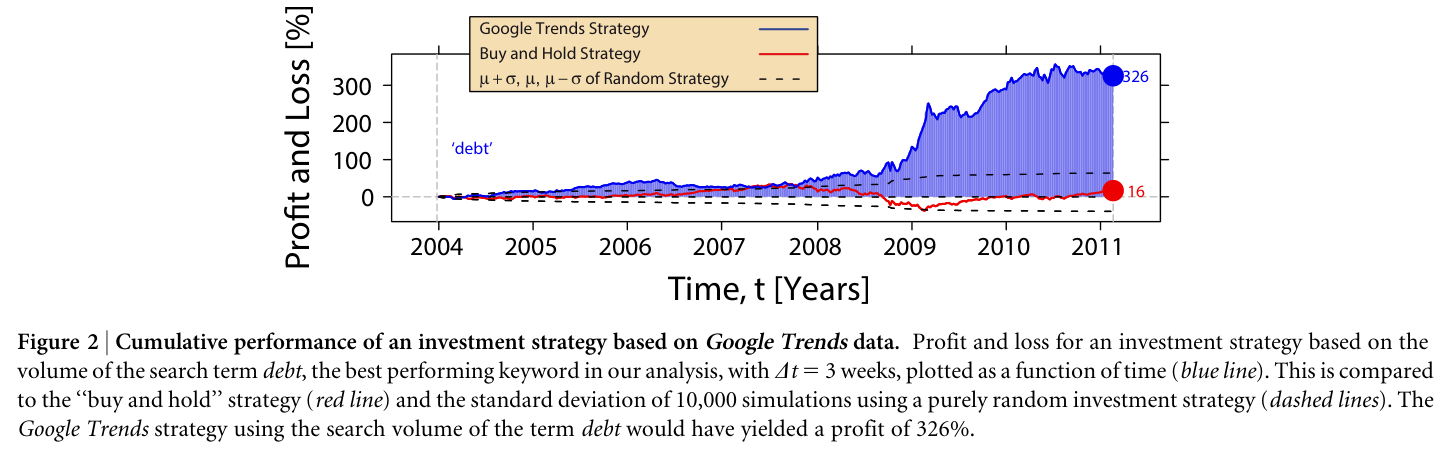
\includegraphics[width=0.8\linewidth]{gfx/m4l2_preis_fig2_cumulative_performance_strategy.png}
\par\smallskip{\small \textbf{Hình 2:} Hiệu suất tích lũy của một chiến lược đầu tư dựa trên dữ liệu Google Trends. Lãi và lỗ của một chiến lược đầu tư dựa trên khối lượng tìm kiếm của từ khóa \emph{debt}, từ khóa cho hiệu suất tốt nhất trong phân tích của chúng tôi, với $\Delta t = 3$ tuần, được biểu diễn theo thời gian (đường màu xanh lam). Kết quả này được so sánh với chiến lược ``mua và nắm giữ'' (đường màu đỏ) và độ lệch chuẩn của 10,000 mô phỏng sử dụng một chiến lược đầu tư hoàn toàn ngẫu nhiên (các đường nét đứt). Chiến lược Google Trends sử dụng khối lượng tìm kiếm của từ khóa \emph{debt} sẽ mang lại lợi nhuận 326\%.}
\end{figure}

Chúng tôi xếp hạng toàn bộ danh sách 98 từ khóa tìm kiếm được nghiên cứu theo hiệu suất giao dịch của chúng khi sử dụng dữ liệu tìm kiếm chỉ của người dùng Hoa Kỳ (Hình 3A) và khi sử dụng dữ liệu khối lượng tìm kiếm được tạo ra trên toàn cầu (Hình 3B). Để đảm bảo tính vững chắc của kết quả, hiệu suất tổng thể của một chiến lược dựa trên một từ khóa tìm kiếm nhất định được xác định là giá trị trung bình của sáu lợi suất thu được với $\Delta t = 1, \ldots, 6$ tuần. Lợi suất của các chiến lược được tính bằng logarit của các thay đổi tương đối trong giá trị danh mục, theo định nghĩa thông thường về lợi suất. Phân bố các giá trị danh mục cuối cùng thu được từ các chiến lược đầu tư ngẫu nhiên gần với phân bố log chuẩn. Do đó, lợi suất tích lũy từ chiến lược đầu tư ngẫu nhiên, được suy ra từ logarit của các giá trị danh mục này, tuân theo phân bố chuẩn, với giá trị trung bình $\langle R \rangle_{\text{RandomStrategy}} = 0$. Ở đây, chúng tôi báo cáo $R$, lợi suất tích lũy của một chiến lược, theo đơn vị độ lệch chuẩn của lợi suất tích lũy của các chiến lược đầu tư ngẫu nhiên không tương quan này.

Chúng tôi nhận thấy rằng lợi suất từ các chiến lược Google Trends mà chúng tôi kiểm định nhìn chung cao hơn đáng kể so với lợi suất từ các chiến lược ngẫu nhiên ($\langle R \rangle_{US} = 0.60$; $t = 8.65$, $df = 97$, $p < 0.001$, kiểm định t một mẫu).

Chúng tôi so sánh hiệu suất của các từ khóa tìm kiếm này với hai chiến lược tham chiếu. Chiến lược ``mua và nắm giữ'' được thực hiện bằng cách mua chỉ số ngay từ đầu và bán ra vào cuối giai đoạn nắm giữ. Chiến lược này mang lại lợi nhuận 16\%, bằng đúng mức tăng tổng thể của giá trị DJIA trong giai đoạn từ tháng 1 năm 2004 đến tháng 2 năm 2011. Chúng tôi tiếp tục xây dựng một ``chiến lược Dow Jones'' bằng cách sử dụng các thay đổi trong $p(t)$ thay cho các thay đổi trong dữ liệu khối lượng tìm kiếm làm cơ sở cho các quyết định mua và bán. Chúng tôi nhận thấy rằng chiến lược này cũng chỉ mang lại 33\% lợi nhuận với $\Delta t = 3$ tuần, hay khi được xác định là giá trị trung bình của sáu lợi suất thu được với $\Delta t = 1, \ldots, 6$ tuần thì tương đương 0.45 độ lệch chuẩn của lợi suất tích lũy của các chiến lược đầu tư ngẫu nhiên không tương quan (Hình 3A và 3B; xem thêm Hình S101 trong Thông tin Bổ sung).

\begin{figure}[H]
\centering
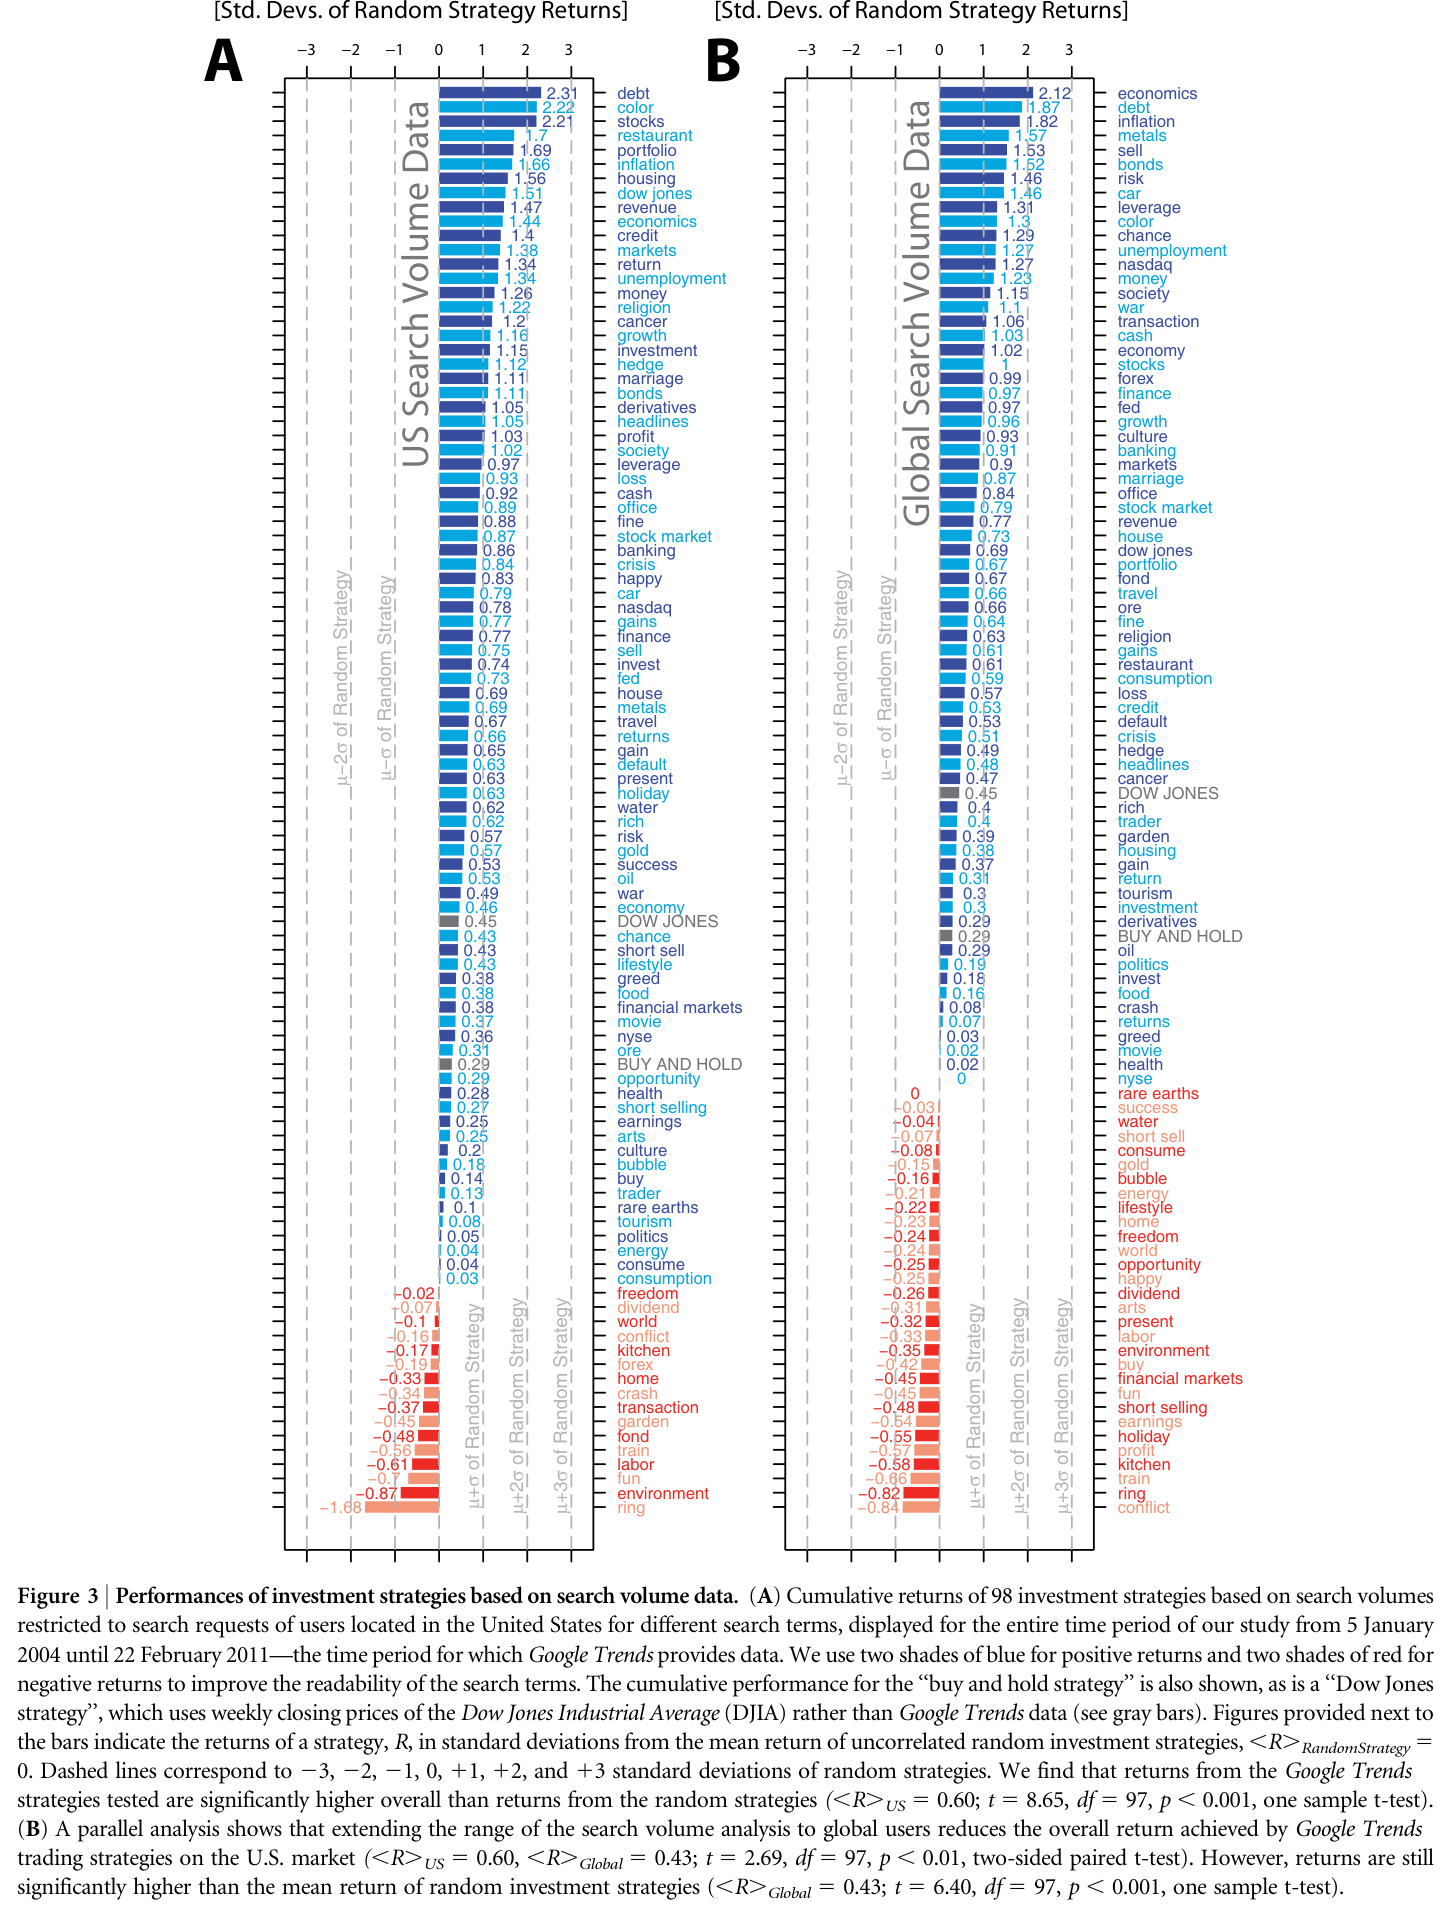
\includegraphics[width=0.8\linewidth]{gfx/m4l2_preis_fig3_performances_search_volume_strategies.png}
\par\smallskip{\small \textbf{Hình 3:} Hiệu suất của các chiến lược đầu tư dựa trên dữ liệu khối lượng tìm kiếm. (A) Lợi suất tích lũy của 98 chiến lược đầu tư dựa trên khối lượng tìm kiếm, giới hạn ở các yêu cầu tìm kiếm của người dùng tại Hoa Kỳ đối với các từ khóa tìm kiếm khác nhau, được trình bày cho toàn bộ giai đoạn nghiên cứu từ ngày 5 tháng 1 năm 2004 đến ngày 22 tháng 2 năm 2011, giai đoạn mà Google Trends cung cấp dữ liệu. Chúng tôi sử dụng hai sắc độ xanh lam cho lợi suất dương và hai sắc độ đỏ cho lợi suất âm nhằm cải thiện khả năng đọc của các từ khóa tìm kiếm. Hiệu suất tích lũy của chiến lược ``mua và nắm giữ'' cũng được trình bày, cùng với ``chiến lược Dow Jones'', chiến lược sử dụng giá đóng cửa hàng tuần của DJIA thay vì dữ liệu Google Trends (xem các thanh màu xám). Các số liệu bên cạnh các thanh thể hiện lợi suất của một chiến lược, $R$, theo đơn vị độ lệch chuẩn so với lợi suất trung bình của các chiến lược đầu tư ngẫu nhiên không tương quan, $\langle R \rangle_{\text{RandomStrategy}} = 0$. Các đường nét đứt tương ứng với $-3, -2, -1, 0, +1, +2$ và $+3$ độ lệch chuẩn của các chiến lược ngẫu nhiên. Chúng tôi nhận thấy rằng lợi suất từ các chiến lược Google Trends được kiểm định nhìn chung cao hơn đáng kể so với lợi suất từ các chiến lược ngẫu nhiên ($\langle R \rangle_{US} = 0.60$; $t = 8.65$, $df = 97$, $p < 0.001$, kiểm định t một mẫu). (B) Một phân tích song song cho thấy việc mở rộng phạm vi phân tích khối lượng tìm kiếm sang người dùng toàn cầu làm giảm lợi suất tổng thể đạt được bởi các chiến lược giao dịch Google Trends trên thị trường Hoa Kỳ ($\langle R \rangle_{US} = 0.60$, $\langle R \rangle_{\text{Global}} = 0.43$; $t = 2.69$, $df = 97$, $p < 0.01$, kiểm định t bắt cặp hai phía). Tuy nhiên, lợi suất vẫn cao hơn đáng kể so với lợi suất trung bình của các chiến lược đầu tư ngẫu nhiên ($\langle R \rangle_{\text{Global}} = 0.43$; $t = 6.40$, $df = 97$, $p < 0.001$, kiểm định t một mẫu).}
\end{figure}

Kết quả của chúng tôi cho thấy hiệu suất của chiến lược Google Trends khác nhau tùy theo từ khóa tìm kiếm được chọn. Chúng tôi tìm hiểu xem liệu những khác biệt về hiệu suất này có thể được giải thích một phần bằng một chỉ báo về mức độ liên quan tài chính của các từ khóa khác nhau hay không, một khái niệm mà chúng tôi định lượng bằng cách tính tần suất xuất hiện của mỗi từ khóa tìm kiếm trên ấn bản trực tuyến của tờ \emph{Financial Times} từ tháng 8 năm 2004 đến tháng 6 năm 2011, được chuẩn hóa theo số kết quả tìm kiếm Google (Google hits) của mỗi từ khóa (xem Hình S2 trong Thông tin Bổ sung). Chúng tôi nhận thấy rằng lợi suất gắn với một từ khóa tìm kiếm nhất định có tương quan với chỉ báo mức độ liên quan tài chính này, sử dụng hệ số tương quan hạng tau của Kendall ($\tau = 0.275$, $z = 4.01$, $N = 98$, $p < 0.001$).

Người ta thường công nhận rằng nhà đầu tư có xu hướng ưu tiên giao dịch trên thị trường trong nước của họ, cho thấy rằng dữ liệu tìm kiếm chỉ của người dùng Hoa Kỳ, như đã sử dụng trong các phân tích trên, sẽ nắm bắt hành vi thu thập thông tin của những người tham gia thị trường chứng khoán Hoa Kỳ tốt hơn so với dữ liệu của người dùng Google trên toàn cầu. Thật vậy, chúng tôi nhận thấy rằng các chiến lược dựa trên dữ liệu khối lượng tìm kiếm toàn cầu kém thành công hơn so với các chiến lược dựa trên dữ liệu khối lượng tìm kiếm của Hoa Kỳ trong việc dự đoán các biến động của thị trường Hoa Kỳ ($\langle R \rangle_{US} = 0.60$, $\langle R \rangle_{\text{Global}} = 0.43$; $t = 2.69$, $df = 97$, $p < 0.01$, kiểm định t bắt cặp hai phía).

Các kết quả thực nghiệm của chúng tôi cho đến nay phù hợp với một giả thuyết gồm hai phần: cụ thể là những đợt tăng giá quan trọng của DJIA được báo trước bởi sự sụt giảm khối lượng tìm kiếm đối với một số từ khóa liên quan đến tài chính nhất định, và ngược lại, những đợt giảm giá quan trọng của DJIA được báo trước bởi sự gia tăng khối lượng tìm kiếm đối với một số từ khóa liên quan đến tài chính nhất định. Tuy nhiên, chiến lược giao dịch của chúng tôi có thể được phân tách thành hai thành phần chiến lược: một thành phần trong đó sự sụt giảm khối lượng tìm kiếm thúc đẩy chúng tôi mua vào (hay nắm giữ vị thế mua), và một thành phần trong đó sự gia tăng khối lượng tìm kiếm thúc đẩy chúng tôi bán ra (hay nắm giữ vị thế bán khống).

Để xác minh rằng cả hai thành phần chiến lược đều đóng vai trò quan trọng trong kết quả của chúng tôi, sao cho chúng tôi có bằng chứng cho cả hai phần của giả thuyết này, chúng tôi xây dựng và kiểm định một chiến lược trong đó chúng tôi chỉ nắm giữ vị thế mua sau khi khối lượng tìm kiếm sụt giảm và không bao giờ nắm giữ vị thế bán khống (Hình 4A), và một chiến lược khác trong đó chúng tôi chỉ nắm giữ vị thế bán khống sau khi khối lượng tìm kiếm gia tăng và không bao giờ nắm giữ vị thế mua (Hình 4B). Chúng tôi nhận thấy rằng lợi suất từ cả hai thành phần của chiến lược Google Trends đều cao hơn đáng kể so với lợi suất từ một chiến lược đầu tư ngẫu nhiên (các chiến lược vị thế mua: $\langle R \rangle_{\text{USLong}} = 0.41$; $t = 11.42$, $df = 97$, $p < 0.001$, kiểm định t một mẫu; các chiến lược vị thế bán khống: $\langle R \rangle_{\text{USShort}} = 0.19$; $t = 5.28$, $df = 97$, $p < 0.001$, kiểm định t một mẫu).

\begin{figure}[H]
\centering
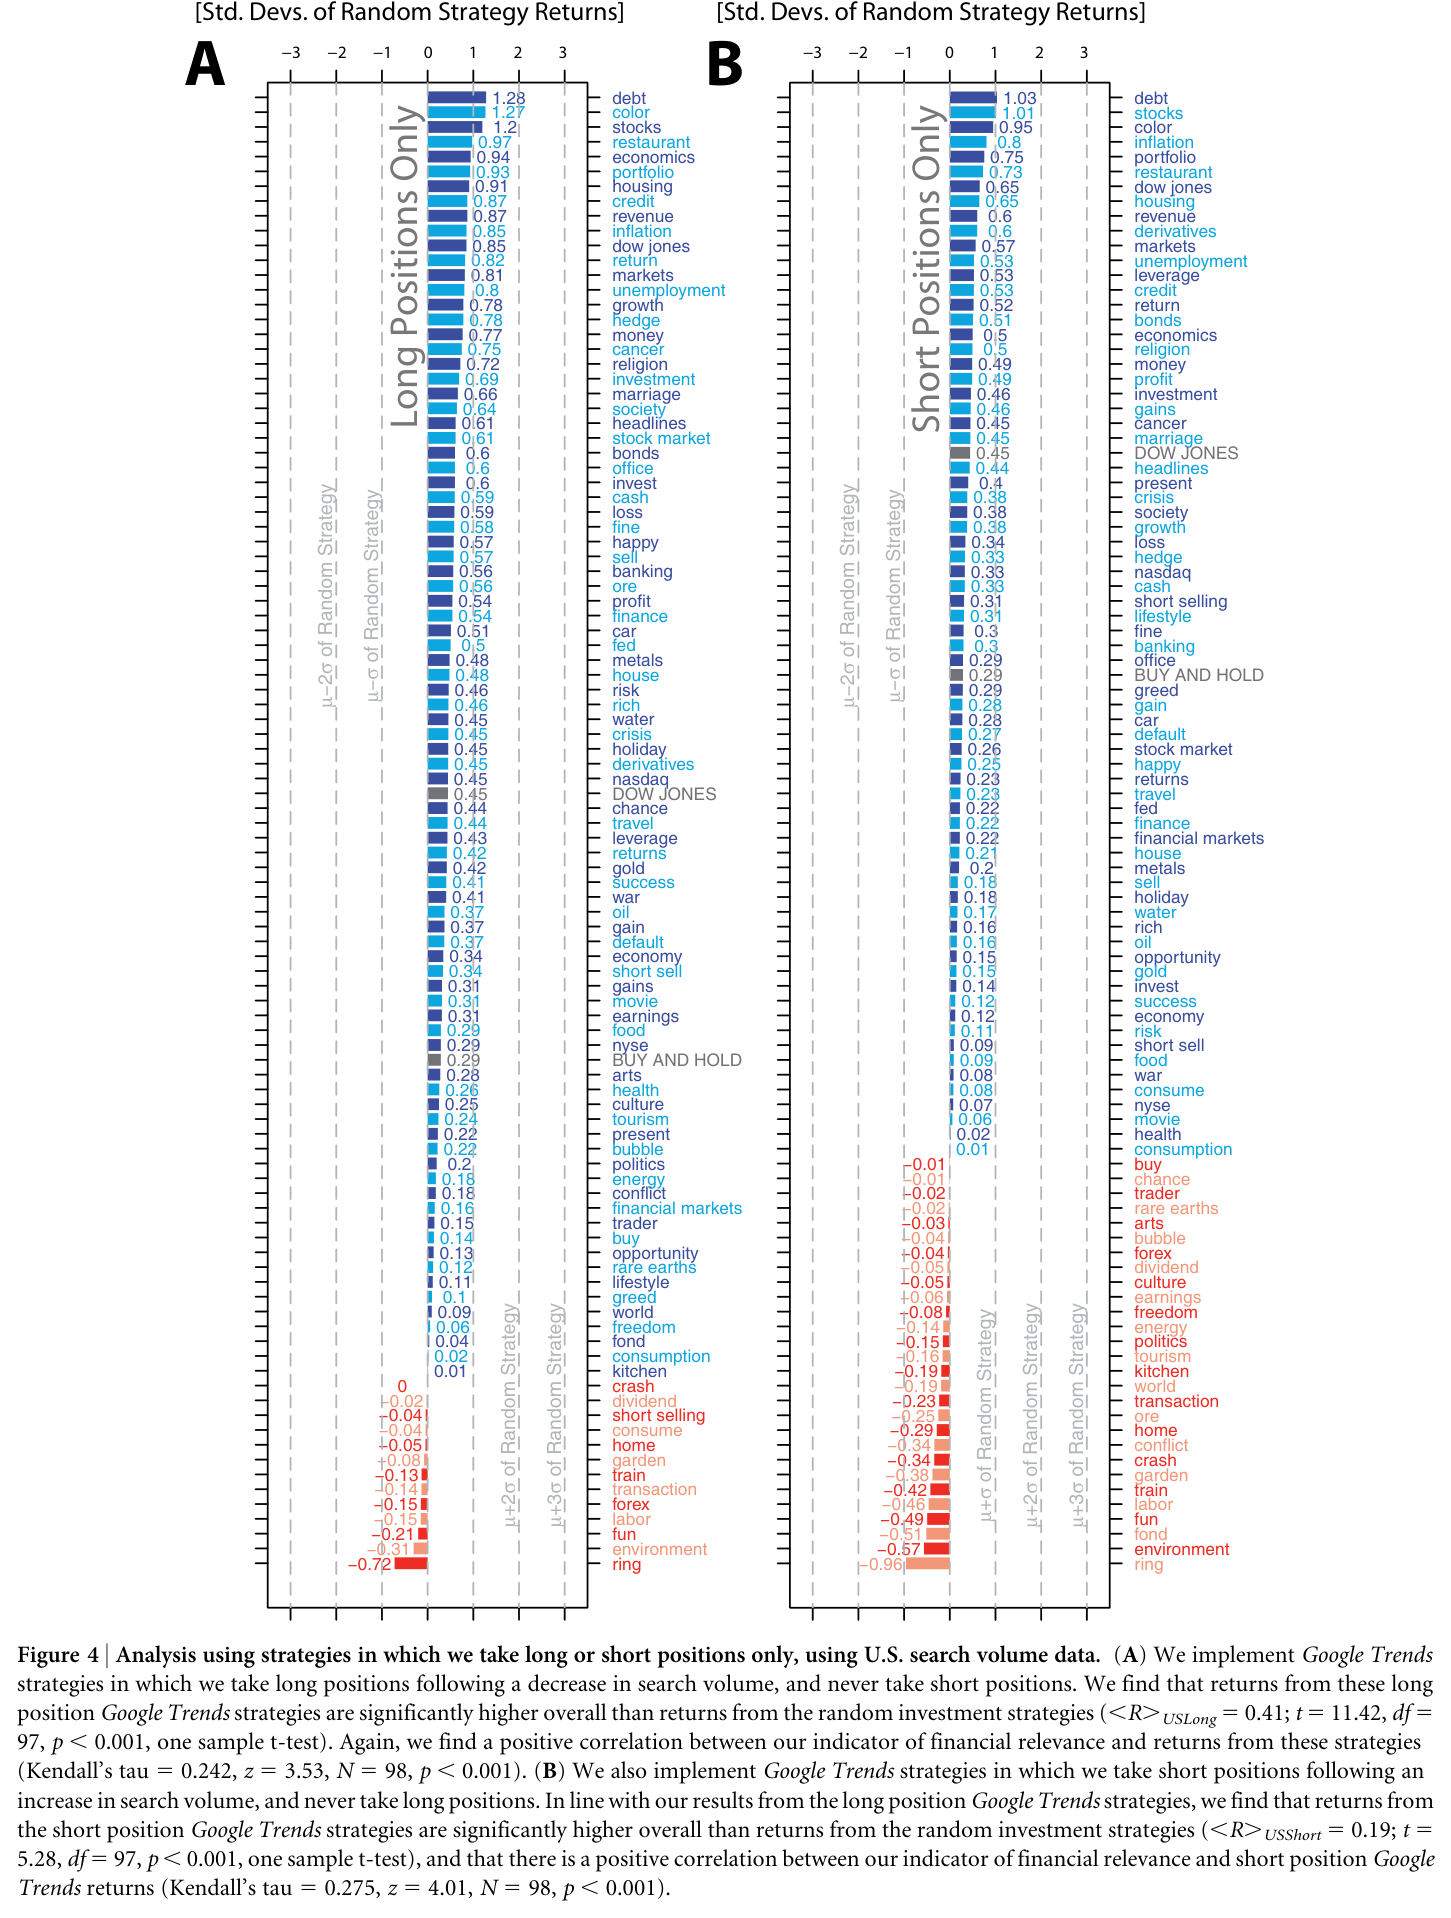
\includegraphics[width=0.8\linewidth]{gfx/m4l2_preis_fig4_long_short_positions_analysis.png}
\par\smallskip{\small \textbf{Hình 4:} Phân tích sử dụng các chiến lược chỉ nắm giữ vị thế mua hoặc vị thế bán khống, sử dụng dữ liệu khối lượng tìm kiếm của Hoa Kỳ. (A) Chúng tôi xây dựng các chiến lược Google Trends trong đó chúng tôi nắm giữ vị thế mua sau một đợt sụt giảm khối lượng tìm kiếm, và không bao giờ nắm giữ vị thế bán khống. Chúng tôi nhận thấy rằng lợi suất từ các chiến lược Google Trends chỉ nắm giữ vị thế mua này nhìn chung cao hơn đáng kể so với lợi suất từ các chiến lược đầu tư ngẫu nhiên ($\langle R \rangle_{\text{USLong}} = 0.41$; $t = 11.42$, $df = 97$, $p < 0.001$, kiểm định t một mẫu). Một lần nữa, chúng tôi tìm thấy mối tương quan dương giữa chỉ báo mức độ liên quan tài chính của chúng tôi và lợi suất từ các chiến lược này (tau Kendall $= 0.242$, $z = 3.53$, $N = 98$, $p < 0.001$). (B) Chúng tôi cũng xây dựng các chiến lược Google Trends trong đó chúng tôi nắm giữ vị thế bán khống sau một đợt gia tăng khối lượng tìm kiếm, và không bao giờ nắm giữ vị thế mua. Phù hợp với kết quả từ các chiến lược Google Trends chỉ nắm giữ vị thế mua, chúng tôi nhận thấy rằng lợi suất từ các chiến lược Google Trends chỉ nắm giữ vị thế bán khống này nhìn chung cao hơn đáng kể so với lợi suất từ các chiến lược đầu tư ngẫu nhiên ($\langle R \rangle_{\text{USShort}} = 0.19$; $t = 5.28$, $df = 97$, $p < 0.001$, kiểm định t một mẫu), và có mối tương quan dương giữa chỉ báo mức độ liên quan tài chính của chúng tôi và lợi suất vị thế bán khống Google Trends (tau Kendall $= 0.275$, $z = 4.01$, $N = 98$, $p < 0.001$).}
\end{figure}

\section{Thảo luận}

Tóm lại, kết quả của chúng tôi phù hợp với gợi ý rằng trong giai đoạn nghiên cứu, dữ liệu Google Trends không chỉ phản ánh các khía cạnh của trạng thái hiện tại của nền kinh tế, mà còn có thể cung cấp một số hiểu biết về các xu hướng tương lai trong hành vi của các chủ thể kinh tế. Sử dụng dữ liệu lịch sử từ giai đoạn tháng 1 năm 2004 đến tháng 2 năm 2011, chúng tôi phát hiện sự gia tăng khối lượng tìm kiếm Google đối với các từ khóa liên quan đến thị trường tài chính trước các đợt sụt giảm của thị trường chứng khoán. Kết quả của chúng tôi cho thấy những dấu hiệu cảnh báo này trong dữ liệu khối lượng tìm kiếm có thể đã được khai thác để xây dựng các chiến lược giao dịch có lợi nhuận.

Chúng tôi đưa ra một cách diễn giải khả dĩ cho kết quả của mình trong khuôn khổ mô hình ra quyết định của Herbert Simon. Chúng tôi cho rằng dữ liệu Google Trends và dữ liệu thị trường chứng khoán có thể phản ánh hai giai đoạn kế tiếp nhau trong quá trình ra quyết định của nhà đầu tư. Xu hướng bán ra trên thị trường tài chính ở mức giá thấp hơn có thể được báo trước bởi các giai đoạn lo ngại. Trong những giai đoạn lo ngại như vậy, con người có thể có xu hướng thu thập thêm thông tin về trạng thái của thị trường. Có thể hình dung rằng hành vi như vậy trước đây có thể đã được phản ánh qua sự gia tăng khối lượng tìm kiếm Google Trends đối với các từ khóa có mức độ liên quan tài chính cao hơn.

Chúng tôi nhận thấy rằng các chiến lược dựa trên dữ liệu khối lượng tìm kiếm của người dùng Hoa Kỳ thành công hơn đối với thị trường Hoa Kỳ so với các chiến lược sử dụng dữ liệu khối lượng tìm kiếm toàn cầu. Với giả định rằng nhóm người dùng Internet tại Hoa Kỳ có tỷ lệ nhà giao dịch trên thị trường Hoa Kỳ cao hơn so với nhóm người dùng Internet trên toàn thế giới, phát hiện này phù hợp với gợi ý thú vị rằng các tập dữ liệu này có thể cung cấp những hiểu biết về các giai đoạn ra quyết định khác nhau trong cùng một nhóm dân số.

Trong công trình này, chúng tôi đưa ra một sự định lượng về mối quan hệ giữa những thay đổi trong khối lượng tìm kiếm và những thay đổi trong giá thị trường chứng khoán. Các nghiên cứu trong tương lai sẽ cần thiết để đưa ra một giải thích thấu đáo về các cơ chế tâm lý nền tảng khiến con người tìm kiếm các từ khóa như \emph{debt} trước khi bán cổ phiếu ở mức giá thấp hơn. Rõ ràng vẫn còn nhiều cơ hội để mở rộng các phân tích của chúng tôi sang các tập dữ liệu tài chính khác.

Kết quả nghiên cứu của chúng tôi cho thấy rằng việc kết hợp các tập dữ liệu hành vi quy mô lớn, chẳng hạn như dữ liệu giao dịch tài chính, với dữ liệu về khối lượng truy vấn tìm kiếm, có thể mở ra những hiểu biết mới về các giai đoạn khác nhau của quá trình ra quyết định tập thể quy mô lớn. Chúng tôi kết luận rằng những kết quả này tiếp tục minh họa cho những khả năng thú vị mà các tập dữ liệu lớn mới mang lại nhằm nâng cao hiểu biết của chúng ta về hành vi tập thể phức tạp trong xã hội.

\section{Phương pháp}

Các từ khóa tìm kiếm liên quan đến chủ đề tài chính ở mức độ nào? Chúng tôi định lượng mức độ liên quan tài chính bằng cách tính tần suất xuất hiện của mỗi từ khóa tìm kiếm trên ấn bản trực tuyến của tờ \emph{Financial Times} (\url{http://www.ft.com}) từ tháng 8 năm 2004 đến tháng 6 năm 2011, được chuẩn hóa theo số kết quả tìm kiếm Google (Google hits, \url{http://www.google.com}) của mỗi từ khóa. Chi tiết được trình bày trong Thông tin Bổ sung.

\textbf{Thu thập dữ liệu.} Chúng tôi thu thập dữ liệu khối lượng tìm kiếm bằng cách truy cập trang web Google Trends (\url{http://www.google.com/trends}) vào các ngày 10 tháng 4 năm 2011, 17 tháng 4 năm 2011 và 24 tháng 4 năm 2011. Dữ liệu về số kết quả tìm kiếm của các từ khóa trên ấn bản trực tuyến của tờ \emph{Financial Times} được thu thập vào ngày 7 tháng 6 năm 2011. Số kết quả tìm kiếm Google (Google hits) cho các từ khóa này được thu thập vào ngày 8 tháng 6 năm 2011.

\section{Lời cảm ơn và thông tin bổ sung}

\textbf{Lời cảm ơn.} Chúng tôi xin cảm ơn Didier Sornette, Dirk Helbing và Steven R. Bishop vì những góp ý của họ. Công trình này được tài trợ một phần bởi Quỹ Nghiên cứu Đức (German Research Foundation), khoản tài trợ PR 1305/1-1 (cho T.P.). Công trình này cũng được hỗ trợ bởi Cơ quan Hoạt động Nghiên cứu Tình báo Tiên tiến (Intelligence Advanced Research Projects Activity, IARPA) thông qua hợp đồng số D12PC00285 của Trung tâm Kinh doanh Quốc gia thuộc Bộ Nội vụ Hoa Kỳ (Department of Interior National Business Center, DoI/NBC), cũng như bởi Quỹ Khoa học Quốc gia (National Science Foundation, NSF), Văn phòng Nghiên cứu Hải quân (Office of Naval Research, ONR) và Cơ quan Giảm thiểu Đe dọa Quốc phòng (Defense Threat Reduction Agency, DTRA). Chính phủ Hoa Kỳ được phép sao chép và phân phối các bản in lại cho các mục đích của Chính phủ, bất kể chú thích bản quyền nào trên đó. Tuyên bố miễn trừ trách nhiệm: các quan điểm và kết luận trong tài liệu này là của các tác giả và không nên được diễn giải là nhất thiết đại diện cho các chính sách hoặc sự chứng thực chính thức, dù được nêu rõ hay ngụ ý, của IARPA, DoI/NBC, hay Chính phủ Hoa Kỳ.

\textbf{Đóng góp của tác giả.} T.P., H.S.M. và H.E.S. đã xây dựng thiết kế nghiên cứu, thực hiện các phân tích, thảo luận về kết quả, và đóng góp vào nội dung của bản thảo.

\textbf{Thông tin bổ sung.} Thông tin bổ sung đi kèm bài báo này tại \url{http://www.nature.com/scientificreports}.

\textbf{Xung đột lợi ích tài chính.} Các tác giả tuyên bố không có xung đột lợi ích tài chính nào.

\textbf{Giấy phép.} Công trình này được cấp phép theo Giấy phép Creative Commons Attribution-NonCommercial-ShareAlike 3.0 Unported. Để xem bản sao của giấy phép này, truy cập \url{http://creativecommons.org/licenses/by-nc-sa/3.0/}.

\textbf{Cách trích dẫn bài báo này:} Preis, T., Moat, H.S. \& Stanley, H.E. Quantifying Trading Behavior in Financial Markets Using Google Trends. \emph{Sci. Rep.} 3, 1684; DOI:10.1038/srep01684 (2013).

% [Đã lược bỏ danh mục Tài liệu tham khảo gốc (tiếng Anh, trích dẫn của tác giả bài gốc) để giảm dung lượng chương; không ảnh hưởng nội dung học thuật chính.]
